In this chapter we will take a look at mathematical models that describe our quadcopter system.

\section{BLDC Motor}
The mathematical model of a BLDC motor is is many ways similar to the one of a conventional DC motor. The main difference is represented by the added phases which affect the resistive and inductive components of the BLDC arrangement.

Therefore, we will start of by describing the mathematical modelling of a DC motor and then change it to fit the BLDC motor.

Figure \label{electromech} illustrates a DC electromechanical system.

\begin{figure}[H]
  \centering
    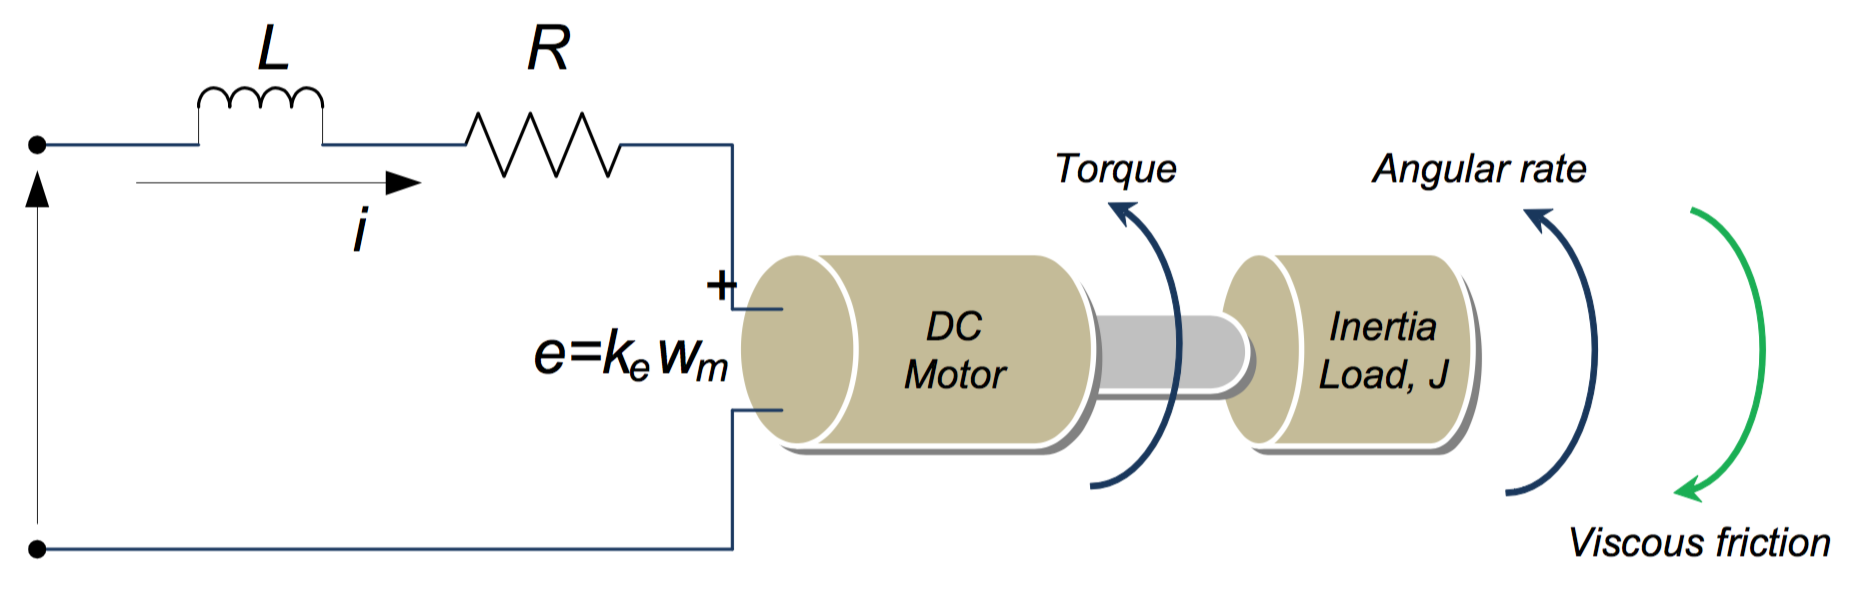
\includegraphics[width=0.9\textwidth]{images/electromech.png}
	\caption{Typical DC electromechanical system}
	\label{electromech}
\end{figure}

The components of the electrical circuit are the armature resistance - R, the armature inductance - L and the back EMF - e. By applying KVL, we obtain:

\begin{equation}
\label{1}
	V_{s}=Ri+L\frac{di}{dt}+e
\end{equation}

where $V_{s}$ - DC source voltage and $i$ - armature current.

Moving on to the mechanical part, further equations can be written using Newton's second law of motion:

\begin{equation}
\label{2}
	J\frac{d\omega_{m}}{dt}=\Sigma{T_{i}}
\end{equation}

\begin{equation}
\label{3}
	T_{e}=k_{f}+J\frac{d\omega_{m}}{dt}+T_{L}
\end{equation}

where $T_{e}$ - electrical torque, $k_{f}$ - friction constant, $J$ - rotor inertia, $\omega_{m}$ - angular velocity and $T_{L}$ - load torque.

The back EMF and the electrical torque can be described as:

\begin{equation}
\label{4}
	T_{e}=k_{t}\omega_{m}
\end{equation}

\begin{equation}
\label{5}
	e=k_{e}\omega_{m}
\end{equation}

where $k_{e}$ - back EMF constant and $k_{t}$ - torque constant.

Rewriting equations \ref{1} and \ref{2} gives:

\begin{equation}
\label{6}
	\frac{di}{dt}=-i\frac{R}{L}-\frac{k_{e}}{L}\omega_{m}+\frac{1}{L}V_{s}
\end{equation}

\begin{equation}
\label{7}
	\frac{d\omega_{m}}{dt}=i\frac{k_{t}}{J}-\frac{k_{f}}{J}\omega_{m}+\frac{1}{J}T_{L}
\end{equation}

Taking the Laplace transform of \ref{6} and \ref{7} yields:

\begin{equation}
\label{8}
	si=i\frac{R}{L}-\frac{k_{e}}{L}\omega_{m}+\frac{1}{L}V_{s}
\end{equation}

\begin{equation}
\label{9}
	s\omega_{m}=i\frac{k_{t}}{J}-\frac{k_{f}}{J}\omega_{m}+\frac{1}{J}T_{L}
\end{equation}

The next equation is obtained by substituting i from equation \ref{9} into \ref{8}.

\begin{equation}
\label{10}
	(\frac{s\omega_{m}+\frac{k_{f}}{J}\omega_{m}-\frac{1}{J}T_{L}}{\frac{k_{t}}{J}})(s+\frac{R}{L})=-\frac{k_{e}}{L}\omega_{m}+\frac{1}{L}V_{s}
\end{equation}  

Assuming there is no load, equation \ref{10} can be rewritten as:

\begin{equation}
\label{11}
	\lbrace{(\frac{s^{2}J}{k_{t}}+\frac{sk_{f}}{k_{t}}+\frac{sRJ}{k_{t}L}+\frac{k_{f}R}{k_{t}L})+\frac{k_{e}}{L}}\rbrace\omega_{m}=\frac{1}{L}V_{s}
\end{equation}

Solving \ref{11} gives:

\begin{equation}
\label{12}
	V_{s}=\frac{s^{2}JL+sk_{f}L+sRJ+k_{f}R+k_{e}k_{t}}{k_{t}}\omega_{m}
\end{equation} 

The transfer function can be obtained as the ratio between the angular velocity $\omega_{m}$ and the source voltage $V_{s}$:

\begin{equation}
\label{13}
	G_{s}=\frac{\omega_{m}}{V_{s}}=\frac{k_{t}}{s^{2}JL+(RJ+k_{f}L)s+k_{f}R+k_{e}k_{t}}
\end{equation} 

Considering that $k_{f}$ tends to zero, the transsfer function can finally be  written as:

\begin{equation}
\label{14}
	G_{s}=\frac{\omega_{m}}{V_{s}}=\frac{k_{t}}{s^{2}JL+RJs+k_{e}k_{t}}
\end{equation} 

In order to obtain the mechanical and electrical time constants, we will need to manipulate equation \ref{14}, which gives:

\begin{equation}
\label{15}
	G_{s}=\frac{\frac{1}{k_{e}}}{\frac{RJ}{k_{e}k_{t}}\frac{L}{R}s^{2}+\frac{RJ}{k_{e}k_{t}}s+1}
\end{equation}

where the mechanical time constant is:

\begin{equation}
\label{16}
	\tau_{m}=\frac{RJ}{k_{e}k_{t}}
\end{equation}

and the electrical time constant is:

\begin{equation}
\label{17}
	\tau_{e}=\frac{L}{R}
\end{equation}

Therefore, substituting equations \ref{16} and \ref{17} into equation \ref{15} yields:

\begin{equation}
\label{18}
	G_{s}=\frac{\frac{1}{k_{e}}}{\tau_{m}\tau_{e}s^{2}+\tau_{m}s+1}
\end{equation}

Equations \ref{15} - \ref{17} will now be changed in order to fit a BLDC motor. Therefore, they will become:

\begin{equation}
\label{19}
	\tau_{m}=\Sigma{\frac{RJ}{k_{e}k_{t}}}=\frac{J\Sigma{R}}{k_{e}k_{t}}
\end{equation}

\begin{equation}
\label{20}
	\tau_{e}=\Sigma{\frac{L}{R}}=\frac{L}{\Sigma{R}}
\end{equation}

Having a symmetrical arrangement and a three phase motor, the constants will finally be:

\begin{equation}
\label{21}
	\tau_{m}=\frac{J3R}{k_{e}k_{t}}
\end{equation}

\begin{equation}
\label{22}
	\tau_{e}=\frac{L}{3R}
\end{equation}

Taking into account the phase effects, $\tau_{m}$ will be rewritten as:

\begin{equation}
\label{23}
	\tau_{m}=\frac{J3R_{\phi}}{k_{e}k_{t}}
\end{equation}

with $k_{e}$ now being the phase value of the back EMF voltage time constant described by:

\begin{equation}
\label{24}
	k_{e}=k_{e(L-L)}/\sqrt{3}
\end{equation}

A relationship between $k_{e}$ - electrical torque and $k_{t}$ - torque constant is found in equation \ref{25}by using the electrical power and mechanical power formulas.

\begin{equation}
\label{25}
	k_{e}=k_{t}\times0.0605
\end{equation}

The next step in coming up with a final transfer function for our motor is to find $\tau_{m}$ and $\tau_{e}$, which are functions of $k_{e}$, $k_{t}$, $R_{\phi}$, J and L. 

A numerical value for $k_{e}$ can be obtained using equation \ref{24}:

\begin{equation}
\label{26}
	k_{e}=\frac{11.1}{1.73}=6.416
\end{equation}

Since $k_{t}$ is a function of $k_{e}$, its numerical value can also be found using equation \ref{25}:

\begin{equation}
\label{27}
	k_{t}=\frac{6.416}{0.0605}=106.04
\end{equation}

For $R_{\phi}$, we have to measure the line-to-line resistance (between any two wires of the motor) and divide the result by 2 in order to get its value.

experiments on J and L / take them from other reports 

\clearpage

\section{Motor Dynamics}
Starting from the top, a brushless motor produces torque given by equation \ref{mmMotor1}.
\begin{equation}
\label{mmMotor1}
	\tau = K_t(I-I_0)
\end{equation}

Here, $\tau$ is the torque, $I$ is the input current, $K_t$ is the constant describing torque proportionality and $I_0$ is the no-load current.

The voltage on the motor is the sum of a resistive loss and the Back-EMF, giving equation \ref{mmMotor2}.
\begin{equation}
\label{mmMotor2}
	V = IR_m + K_\upsilon \omega
\end{equation}
where $V$ is the voltage across the motor, $R_m$ is the motor resistance, $\omega$ is the angular velocity and $K_\upsilon $ is a constant, describing the back-EMF generated per $RPM$.
We can then combine equations \ref{mmMotor1} and \ref{mmMotor2} and put them into the power equation, to get a new equation \ref{mmMotor3}.
\begin{equation}
\label{mmMotor3}
	P = IV = \frac{(\tau + K_tI_0)(K_tI_0R_m + \tau R_m + K_tK_\upsilon \omega)}{K_t^2}
\end{equation}

To help simplify the model, we can assume that the motor resistance is very small and therefore can be disregarded. This gives us a new power equation \ref{mmMotor4}.
\begin{equation}
\label{mmMotor4}
	P \approx \frac{(\tau + K_tI_0)K_\upsilon \omega}{K_t}
\end{equation}

We can also, for the purposes of simplifying the model, assume that $K_tI_0\ll \tau$. This is a reasonable assumption due to the fact that $I_0$ describes the current with no load on the motor and is usually a small number. Based on this, we can then obtain the final equation \ref{mmMotor5} for power.
\begin{equation}
\label{mmMotor5}
	P \approx \frac{K_\upsilon }{K_t}\tau \omega
\end{equation}

From the conservation of energy, it is known that the energy that the motor expends during some period of time is equal to the force generated by the propeller multiplied by the distance the it displaces moves, given by the equation \ref{mmMotor6}.
\begin{equation}
\label{mmMotor6}
	P\times dt = F\times dx
\end{equation}
We can then say that the power is also equal to the thrust multiplied by the air velocity, as seen in equation \ref{mmMotor7}.
\begin{equation}
\label{mmMotor7}
	P = F\frac{dt}{dx} = T\upsilon _h
\end{equation}
Here - $T$ is the thrust and $\upsilon _h$ is the air velocity. Since the model is describing a hovering quadcopter in a closed area, only $\upsilon _h$ is an acting velocity (i.e. vehicle speed has no effect and free stream velocity is equal to zero).

Momentum theory gives equation \ref{mmMotor8}, for the hover velocity $\upsilon _h$.
\begin{equation}
\label{mmMotor8}
	\upsilon _h = \sqrt{\frac{T}{2\rho A}}
\end{equation}

where $A$ is the area swept out by the blade and $\rho$ is the air density.
In the case of this model, $\tau$ is proportional to thrust $T$ by a constant $K_\tau$. Keeping this in mind, we can now use the simplified power equation \ref{mmMotor5} and derive a new equation \ref{mmMotor9}.
\begin{equation}
\label{mmMotor9}
 	P = \frac{K_\upsilon }{K_t}\tau \omega = \frac{K_\upsilon K_\tau }{K_t}T\omega = \frac{F^{\frac{3}{2}}} {\sqrt{2\rho A}}
\end{equation}

Solving for thrust $T$, we can derive a new equation \ref{mmMotor10}.
\begin{equation}
\label{mmMotor10}
 	T = (\frac{K_\upsilon K_\tau \sqrt{2\rho A}}{K_t}\omega)^2 = k\omega ^2
\end{equation}

where $k$ is a constant, describing all other constants used in the equation.

The final equation \ref{mmMotor10} now describes the thrust $T$ generated by the motor with angular velocity $\omega$ as an input.